\documentclass[11pt]{article}

\usepackage[margin=1in]{geometry}
\usepackage{amsmath,amssymb,amsthm}
\usepackage{mathtools}
\usepackage{booktabs}
\usepackage{tikz}
\usepackage{hyperref}

\theoremstyle{plain}
\newtheorem{theorem}{Theorem}
\newtheorem{lemma}{Lemma}

\theoremstyle{definition}
\newtheorem{definition}{Definition}

\title{A Rank-Count Theory for the Combinatorial Discretizable Distance Geometry Problem}
\author{
Michael Souza\\
Universidade Federal do Cear\'a\\
\texttt{michael@ufc.br}
\and
Wagner da Rocha\\
Unicamp\\
\texttt{wdarocha@ime.unicamp.br}
\and
Carlile Lavor\\
Unicamp\\
\texttt{clavor@unicamp.br}
}
\date{}

\begin{document}

\maketitle

\begin{abstract}
The Combinatorial Discretizable Distance Geometry Problem (Combinatorial DDGP)
uses a vertex order where every reference predecessor set induces a clique to
discretize graph realizations via Branch-and-Prune. In this subclass, the
number of realizations is almost always \(2^{n-K}\) when no pruning edges are
present. In the presence of pruning edges, a topological count has remained
elusive; prior work only conjectured a count using contractions on the
\(K\)-incident graph, leaving the formal proof to future research. We develop
an algebraic rank-count theory for the feasible binary Branch-and-Prune codes.
Branch transformations are encoded by graph-derived generators, and their
conflicts with pruning constraints are recorded in a labeled violation matrix.
Under generic mirror separation, the feasible codes form an affine space over
\(\mathbb{F}_2\). The number of realizations is therefore given by a rank
formula, with one factor of two for each branch decision not constrained by
pruning. The formula recovers the classical \(2^{n-K}\) count when no pruning
edges are present.
\end{abstract}

\section{Introduction}
\label{sec:intro}

This paper studies solution counting for ordered Combinatorial Discretizable Distance Geometry Problem (Combinatorial DDGP) instances with pruning edges. Fix a predecessor system and let \(B=V\setminus V_0\) be the binary Branch-and-Prune decision set, where \(V_0=\{v_1,\ldots,v_K\}\) is the initial clique. Pruning edges determine a constrained branch set \(B_{\mathrm{c}}\subseteq B\); the remaining \(f=\lvert B\setminus B_{\mathrm{c}}\rvert\) branch decisions are free. We prove that, under a generic mirror-separation hypothesis and relative to any reference solution, the feasible codes on \(B_{\mathrm{c}}\) form an affine space over \(\mathbb{F}_2\). Consequently, the number of feasible full branch codes is
\[
2^{
f+
\operatorname{rank}_{\mathbb{F}_2}\begin{bmatrix} M \\ V \end{bmatrix}
-
\operatorname{rank}_{\mathbb{F}_2}(V)
},
\]
where \(M\) is the graph-derived branch-generator matrix and \(V\) is the labeled violation matrix for pruning constraints.

The Distance Geometry Problem (DGP) asks for a geometric representation of a weighted graph in $\mathbb{R}^K$: given a simple undirected graph $G = (V, E)$ and an edge weight function $d: E \to \mathbb{R}_+$, find an embedding $x: V \to \mathbb{R}^K$ such that $\|x_i - x_j\|_2 = d_{ij}$ for every $\{i,j\}\in E$~\cite{mucherino2012discretizable}. The problem appears in protein structure determination from nuclear magnetic resonance (NMR) distance data~\cite{liberti2008branch}, sensor network localization~\cite{abud2018k}, and the geometry of nanostructures~\cite{mucherino2020analysis}.

When a vertex order on $V = \{1, \ldots, n\}$ is part of the input, the search space can be discretized. In DDGP and DMDGP instances~\cite{mucherino2012discretizable,lavor2012discretizable}, each non-seed vertex $j > K$ has a predecessor set $U_j \subset \{1, \ldots, j-1\}$ of size $K$. Once the predecessors are placed, $K$-lateration determines the position of $j$ as the intersection of $K$ spheres centered at the predecessor coordinates~\cite{liberti2014number}. Generically, this intersection contains at most two points, organizing realizations as paths in the Branch-and-Prune (BP) tree~\cite{liberti2008branch}.

We naturally partition the edges in $G$ into two sets:
\begin{enumerate}
    \item \textbf{Discretization edges} ($E_D = \{\{i, j\} \in E \mid i \in U_j\}$), which we use to perform the $K$-lateration steps and branch into the binary tree.
    \item \textbf{Pruning edges} ($E_P = E \setminus E_D$), which represent additional distance constraints that the BP algorithm uses to check the feasibility of branched positions and prune inconsistent paths in the tree.
\end{enumerate}

General DDGP counting cannot be purely graph-combinatorial in the unrestricted sense: numerical edge weights can change the number of feasible branches~\cite{abud2024impossible}. In the Combinatorial DDGP, the predecessor cliques restore enough reflection structure to make a rank count possible after pruning constraints are labeled by their relevant mirrors. The generic mirror-separation assumption excludes the proper algebraic exceptional set where a geometrically violating transformation accidentally preserves a distance. Outside this set, the feasible branch differences are exactly the zero-violation shifts.

Throughout the paper, all branch codes, vector spaces, sums, kernels, and ranks are over the finite field $\mathbb{F}_2$.

Our contribution is threefold:
\begin{enumerate}
    \item We decompose the branch decisions into pruning-constrained and pruning-free bits, and represent constrained branch transformations using graph-derived cone generators and base generators.
    \item We introduce a labeled violation matrix that separates violations caused by different mirror cliques, keeping track of mirror-specific incompatibilities.
    \item We prove the \emph{Rank-Count Theorem}: relative to any reference solution $s^\ast$, the feasible constrained branch codes form an affine coset with direction $\mathcal{K}_F$, the space of zero-violation shifts. Consequently,
    \[
    \lvert \Xi \rvert
    =
    2^{f+\operatorname{rank}_{\mathbb{F}_2}\begin{bmatrix} M \\ V \end{bmatrix} - \operatorname{rank}_{\mathbb{F}_2}(V)},
    \]
    where $M$ is the generator mask matrix and $V$ is the labeled violation matrix.
\end{enumerate}

Binary branch-code representations are standard for paths in the Branch-and-Prune tree; related binary representations have been widely used to analyze symmetry and degrees of freedom in distance geometry~\cite{mucherino2012exploiting,mucherino2020analysis}.

We organize the remainder of the paper as follows. Section~\ref{sec:related} reviews DMDGP symmetries, Combinatorial DDGP counts, DDGP recognition, and the counting barrier for general DDGP instances. Sections~\ref{sec:subproblems}--\ref{sec:shifts} define branch codes, generators, labeled violations, and feasible branch shifts. Section~\ref{sec:results} proves the main theorem. Section~\ref{sec:example} gives a fully worked 6-vertex example. Section~\ref{sec:scope} discusses scope, genericity, and the no-pruning Combinatorial DDGP special case.

\section{Related Work}
\label{sec:related}

We review three strands of prior work used below: DMDGP partial-reflection symmetry, DDGP recognition, and the negative counting result for general DDGP instances.

In the DMDGP, the predecessor sets $U_j$ are contiguous and immediately precede $j$ in the vertex order, so $U_j = \{j-K, \ldots, j-1\}$~\cite{lavor2012discretizable}. This contiguity ensures that each $U_j$ induces a clique of size $K$ in $G$. The clique property implies that the branch choices at each level are partial reflections across affine hyperplanes spanned by predecessor coordinates~\cite{mucherino2012exploiting}. These reflections form a group of partial-reflection symmetries acting on the BP tree. They explain the generic power-of-two solution counts and the structure of the search space~\cite{liberti2011number,liberti2014number}. 

Because these reflections act on suffix intervals of the vertex order, one can count the number of feasible BP paths by a combinatorial method depending on graph topology rather than numerical edge weights~\cite{lavor2021optimality}. This counting method has been used to prove fixed-parameter tractability of the BP algorithm on DMDGP instances with respect to $K$ and a branching-frequency parameter $v_0$. Partial-reflection symmetries also support build-up, splitting, and search algorithms for DMDGP instances~\cite{mucherino2012exploiting,goncalves2021new}. 

Finding a valid DMDGP vertex order from a graph is NP-complete for any fixed dimension $K \ge 2$~\cite{cassioli2015discretization}. In the general DDGP, the predecessor sets $U_j$ need not be consecutive. This relaxation changes the computational tradeoff: finding a valid DDGP order can be done in polynomial time by an FPT algorithm with respect to $K$~\cite{abud2024impossible}. 

The same relaxation complicates counting. Since DDGP predecessors are not necessarily consecutive, reflections no longer act on suffix intervals. A branch change at a vertex $q$ propagates through a directed dependency graph of successors. This dynamic propagation is the obstruction we address in the present local construction.

Abud et~al.~\cite{abud2024impossible} proved that no purely combinatorial counting method exists for the general DDGP. Their 5-vertex counterexample has a predecessor set $U_5 = \{1,4\}$ that does not induce a clique. After branching on vertex 4, one candidate coordinate for vertex 5 can violate the triangle inequality on $\{1,4,5\}$ with positive probability. Thus the number of valid coordinates for vertex 5, and therefore the total solution count, depends on the numerical edge weights rather than only on graph topology. Our result does not contradict this barrier: it gives a generic rank count for a fixed local active subproblem, not a global combinatorial count for arbitrary DDGP instances.

\section{Branch Codes and Pruning Constraints}
\label{sec:subproblems}

We now define the branch-code space for the whole ordered instance and isolate the branch decisions that can affect pruning constraints.

Let the vertices be ordered as $v_1,\ldots,v_n$, and write $U_i$ for the predecessor set of $v_i$. When a vertex $q=v_i$ appears as a subscript, $U_q$ means $U_i$; this preserves the paper's vertex notation while making the order explicit.

Let $V_0=\{v_1,\ldots,v_K\}$ be the fixed initial clique in $\mathbb{R}^K$. For $i\le K$, set $U_i=\varnothing$. For every non-seed vertex $i > K$, the predecessor set $U_i \subseteq \{v_1,\ldots,v_{i-1}\}$ has size $K$. The predecessor relation defines a directed acyclic graph with an arc $v_j \to v_i$ whenever $v_j \in U_i$.

Related order-dependent reference structures have been studied through $K$-discretization and $K$-incident graphs~\cite{abud2018k}; here we fix one predecessor system and derive branch shifts from its dependency cones.

\begin{definition}[Fixing set]
\label{def:fixing}
The fixing set of a vertex $v_i$ is
\[
\operatorname{Fix}_U(v_i)
=
\{v_i\}\cup \bigcup_{u\in U_i}\operatorname{Fix}_U(u).
\]
For seed vertices this gives the base case $\operatorname{Fix}_U(v_i)=\{v_i\}$ because $U_i=\varnothing$.
\end{definition}

\begin{definition}[Dependency cone]
\label{def:cone}
The dependency cone of a vertex $v_i$ is
\[
\operatorname{Cone}_U(v_i)
=
\{v_i\}\cup \bigcup_{w:\,v_i\in U_w}\operatorname{Cone}_U(w),
\]
where $w$ ranges over vertices. If no later vertex has $v_i$ as a predecessor, this gives the terminal base case $\operatorname{Cone}_U(v_i)=\{v_i\}$.
\end{definition}

Let $E_D$ denote the discretization edges induced by the predecessor relation, and let $E_P = E\setminus E_D$ denote the pruning edges. The full branch-decision set is
\[
B = V\setminus V_0.
\]
Define the pruning-relevant vertex set
\[
L
=
\bigcup_{\{u,v\}\in E_P}
\left(\operatorname{Fix}_U(u)\cup \operatorname{Fix}_U(v)\right),
\]
and the pruning-constrained branch set
\[
B_{\mathrm{c}}=L\setminus V_0.
\]
The remaining branch decisions
\[
B_{\mathrm{f}}=B\setminus B_{\mathrm{c}},
\qquad
f=\lvert B_{\mathrm{f}}\rvert,
\]
are free with respect to pruning constraints: changing them preserves all discretization edges by construction and cannot change the endpoints of any pruning edge.

The constrained edge set is
\[
F = E_D[L] \cup E_P,
\qquad
E_D[L]=\{\{u,v\}\in E_D \mid u,v\in L\}.
\]
When $E_P=\varnothing$, we have $L=\varnothing$, $B_{\mathrm{c}}=\varnothing$, and all branch decisions are free.

Let $x(s)=(x_a(s))_{a\in V}$ denote the embedding determined by the full branch code $s\in\mathbb{F}_2^B$. The full solution code is
\[
\Xi
=
\{s \in \mathbb{F}_2^B \mid
\|x_a(s)-x_b(s)\|_2=d_{ab}
\text{ for every } \{a,b\}\in E\}.
\]
The constrained solution code is
\[
\Xi_F
=
\{s_{\mathrm{c}} \in \mathbb{F}_2^{B_{\mathrm{c}}} \mid
\|x_a(s)-x_b(s)\|_2=d_{ab}
\text{ for every } \{a,b\}\in F\},
\]
where $s$ is any full branch code whose restriction to $B_{\mathrm{c}}$ is $s_{\mathrm{c}}$. This is well-defined because branch decisions in $B_{\mathrm{f}}$ do not affect edges in $F$. Hence
\[
\lvert \Xi\rvert = 2^f \lvert \Xi_F\rvert.
\]
Our goal is to compute $\lvert \Xi\rvert$ under generic geometric assumptions without running tree-based branch search.

\section{Graph-Derived Generators}
\label{sec:generators}

This section defines the graph-derived generators that encode branch transformations and their mirror cliques. We use cone generators for dependency propagation, base generators for common predecessor cliques, and the mask matrix to project generator combinations to branch masks.

A generator represents a branch transformation together with the mirror clique that explains its geometric action. Each generator is a pair
\[
g=(m_g, C_g),
\]
where $m_g \in \mathbb{F}_2^{B_{\mathrm{c}}}$ is a branch mask and $C_g$ is a predecessor clique. The mask tells which pruning-constrained branch bits are toggled; the clique tells which affine mirror is used for the reflection.

\begin{definition}[Cone generator]
\label{def:cone-generator}
For each decision vertex $q \in B_{\mathrm{c}}$, the cone generator is
\[
g_q = (m_q, U_q),
\qquad
\operatorname{supp}(m_q) = B_{\mathrm{c}} \cap \operatorname{Cone}_U(q).
\]
\end{definition}

When the rows and cone-generator columns are ordered by the DDGP vertex order, the cone-mask matrix is triangular with diagonal entries equal to one. Hence the cone masks $\{m_q \mid q\in B_{\mathrm{c}}\}$ form a basis of the constrained branch space $\mathbb{F}_2^{B_{\mathrm{c}}}$.

The predecessor-clique set used for base generators is
\[
\mathcal{C}_{\mathrm{c}}=\{U_w\mid w\in B_{\mathrm{c}}\}.
\]

\begin{definition}[Base generator]
\label{def:base-generator}
For a predecessor clique $C\in\mathcal{C}_{\mathrm{c}}$, define the generator roots:
\[
\operatorname{Gen}_{\mathrm{c}}(C)=\{w \in B_{\mathrm{c}} \mid U_w = C\}.
\]
The base generator associated with $C$ is
\[
g_C=(m_C, C),
\]
where
\[
\operatorname{supp}(m_C)
=
B_{\mathrm{c}} \cap \bigcup_{w:\,U_w=C} \operatorname{Cone}_U(w)
=
\bigcup_{w\in \operatorname{Gen}_{\mathrm{c}}(C)} \operatorname{supp}(m_w).
\]
\end{definition}

Base generators are useful because two transformations with the same branch mask may have different geometric meaning if they use different mirror cliques. Thus, a base generator may be redundant as a column of the mask matrix while still being necessary as a labeled geometric operation.

After defining both kinds of generators, set $\mathcal{G}$ to be the labeled generator family
\[
\mathcal{G}
=
\{g_q\mid q\in B_{\mathrm{c}}\}\sqcup\{g_C\mid C\in\mathcal{C}_{\mathrm{c}}\},
\qquad
m=\lvert\mathcal{G}\rvert.
\]
This is an indexed family of generator columns, not a quotient by branch mask. Duplicate masks are retained as separate columns when they carry distinct cone or base labels, and in particular when they carry distinct mirror labels. The generator coefficient space is
\[
A = \mathbb{F}_2^{\mathcal{G}}.
\]
Choose an enumeration $\mathcal{G}=\{g^1,\ldots,g^m\}$ for the matrix representation below.

\begin{definition}[Mask matrix]
\label{def:mask-matrix}
The generator mask matrix is the linear map
\[
M: A \to \mathbb{F}_2^{B_{\mathrm{c}}},
\]
whose $j$-th column is $m_{g^j}$. For any generator coefficient vector $\alpha=(\alpha_1,\ldots,\alpha_m)\in A$, the action of $M$ is
\[
M\alpha = \bigoplus_{g^j:\,\alpha_j = 1} m_{g^j}.
\]
\end{definition}

The vector $M\alpha$ represents the net branch mask produced by the generator combination $\alpha$.

\section{Labeled Violations}
\label{sec:violations}

The mask $m_g$ tells which branch bits change, but it does not by itself say which distances are preserved. Geometrical distance preservation depends on the mirror clique attached to the transformation.

Fix the active edge set $F$. Let $g=(m_g,C_g)$ be a generator, and write
\[
S_g = \operatorname{supp}(m_g).
\]
An active edge $e = \{a,b\} \in F$ crosses the support boundary of $g$ if exactly one endpoint is toggled:
\[
|e \cap S_g| = 1.
\]
If this happens, one endpoint is moved by the reflection while the other is fixed. The edge length is preserved only when the fixed endpoint lies on the reflection mirror, which is ensured when it belongs to $C_g$. Therefore, we say that $g$ violates $e$ if
\[
|e \cap S_g| = 1
\quad\text{and}\quad
e\setminus S_g \not\subseteq C_g.
\]
Because $e$ crosses the support boundary, the set difference $e \setminus S_g$ is a singleton containing the unique endpoint of $e$ that remains fixed. The condition $e \setminus S_g \not\subseteq C_g$ is therefore equivalent to saying that this fixed endpoint does not belong to the mirror clique $C_g$, which geometrically means that the fixed endpoint does not lie on the reflection mirror hyperplane $\operatorname{aff}(C_g)$.

Violations are labeled by both the edge and the mirror clique. Let
\[
\mathcal L
=
\{(e,C_g) \mid g \in \mathcal G,\ e \in F,\ g\text{ violates }e\}.
\]
The labeled violation matrix is the linear map
\[
V: A \to \mathbb{F}_2^{\mathcal L}.
\]
Rows are indexed by labeled pairs $\ell_i=(e_i,C_i)\in\mathcal L$, and columns are indexed by generators $g^j$. Its entries are
\[
V_{ij} = 1
\quad\Longleftrightarrow\quad
C_i = C_{g^j} \text{ and } g^j \text{ violates } e_i.
\]
Thus, $V\alpha$ represents the net labeled violation pattern of the generator combination $\alpha$. The same active edge may be crossed by transformations using different predecessor mirrors; such violations are kept in distinct rows and cannot cancel unless their mirror labels agree.

\section{Feasible Branch Shifts}
\label{sec:shifts}

This section formalizes the concept of the feasible branch shift space, which characterizes the coordinate transformations that preserve active distance constraints. 
Geometrically, moving from a branch code $s$ to $s \oplus h$ via a branch shift $h \in \mathbb{F}_2^{B_{\mathrm{c}}}$ corresponds to a sequence of partial reflections. 
A shift preserves the validity of all active constraints if it is produced by a generator combination with zero net violations, meaning $\alpha \in \ker V$. 
Because multiple generator combinations can yield the same branch mask, the space of valid branch shifts $\mathcal{K}_F$ is defined as the image of this kernel under the mask matrix $M$:
\[
\mathcal{K}_F = M(\ker V).
\]
To ensure that only shifts within $\mathcal{K}_F$ preserve these distances under generic geometric configurations, we introduce the \emph{generic mirror separation} hypothesis.

\begin{definition}[Generic mirror separation]
\label{def:mirror-sep}
Let $P$ be the real algebraic set of nondegenerate lateration parameters (predecessor coordinates and active edge lengths). 
The instance satisfies generic mirror separation if there exists a proper algebraic exceptional set $Z \subset P$ such that, for all parameters in $P \setminus Z$, any shift $h \notin \mathcal{K}_F$ and branch code $s$ satisfy
\[
\|x_a(s \oplus h) - x_b(s \oplus h)\|_2 \neq \|x_a(s) - x_b(s)\|_2
\]
for at least one active edge $\{a,b\} \in F$ (where both embeddings are defined).
\end{definition}

We use generic mirror separation as an explicit instance-level hypothesis. The main theorem below does not assert that every ordered instance satisfies it; rather, it proves the rank count for instances that do.

The next section uses this hypothesis to prove the algebraic rank count.

\section{Main Results}
\label{sec:results}

We now prove the rank-count theorem. First, a linear-algebra lemma computes the dimension of the projected zero-violation space. Then a preservation lemma gives the geometric implication of zero labeled violation. Finally, the main theorem identifies the whole local solution code as an affine shift of that space.

\begin{lemma}[Branch-shift rank]
\label{lem:rank}
For the feasible branch shift space $\mathcal{K}_F = M(\ker V)$,
\[
\dim \mathcal{K}_F
=
\operatorname{rank}\begin{bmatrix} M \\ V \end{bmatrix}
-
\operatorname{rank}(V).
\]
\end{lemma}

\begin{proof}
Let $m = \lvert \mathcal{G} \rvert = \dim A$. Since $\mathcal{K}_F = M(\ker V)$, we restrict $M$ to $\ker V$:
\[
M\big|_{\ker V} : \ker V \to \mathbb{F}_2^{B_P}.
\]
By rank-nullity applied to this restricted map,
\[
\dim \mathcal{K}_F
=
\dim \ker V
-
\dim(\ker V \cap \ker M).
\]
Now $\dim \ker V = m - \operatorname{rank}(V)$, and
\[
\ker V \cap \ker M
=
\ker\begin{bmatrix} M \\ V \end{bmatrix}.
\]
Therefore,
\[
\dim(\ker V \cap \ker M)
=
m - \operatorname{rank}\begin{bmatrix} M \\ V \end{bmatrix}.
\]
Substituting these dimensions into the rank-nullity equation gives:
\[
\begin{aligned}
\dim \mathcal{K}_F &= (m - \operatorname{rank}(V)) - \left(m - \operatorname{rank}\begin{bmatrix} M \\ V \end{bmatrix}\right) \\
&= \operatorname{rank}\begin{bmatrix} M \\ V \end{bmatrix} - \operatorname{rank}(V).
\end{aligned}
\]
This completes the proof.
\end{proof}

The next lemma is the geometric direction encoded by the labeled violation matrix: zero net labeled violation gives a composition of mirror-compatible blocks, hence preserving every active edge.

\begin{lemma}[Zero-violation preservation]
\label{lem:preservation}
Let $\alpha \in \ker V$ and let $h = M\alpha$. If $s \in \Xi_F$, then $s \oplus h \in \Xi_F$.
\end{lemma}

\begin{proof}
We group the selected generators in $\alpha$ by mirror clique. For a fixed clique $C$, let $S_C$ be the XOR of the supports of the selected generators with mirror $C$. The row $(e,C)$ of $V\alpha$ represents the parity of selected generators with mirror $C$ that violate the active edge $e$. We have $V\alpha = 0$. Therefore, this parity is zero for every active edge $e \in F$ and every mirror clique $C$.

Therefore, the block $(S_C, C)$ is mirror-compatible with each active edge: if an active edge crosses $S_C$, its fixed endpoint lies in $C$. Generator supports are disjoint from their own mirror clique. Consequently, an endpoint in $C$ is never moved by a generator with mirror $C$. If a crossing edge had its fixed endpoint outside $C$, the selected generators with mirror $C$ would contribute an odd violation parity to the row $(e,C)$. This contradicts $V\alpha = 0$.

Reflection through the affine span $\operatorname{aff}(C)$ preserves edges with both endpoints moved, edges with neither endpoint moved, and crossing edges whose fixed endpoint lies directly on the mirror. Although spatial reflections generally do not commute, here any active edge crossing the block support $S_C$ has its fixed endpoint lying directly on the mirror $\operatorname{aff}(C)$. Consequently, each block reflection acts symmetrically on active edges, preserving the coordinates and affine hyperplanes representing subsequent mirror cliques. The composition of these reflections is therefore well-defined, and applying these block reflections one mirror clique at a time preserves every edge in $F$. Their net branch mask is $\bigoplus_C S_C = M\alpha = h$. Thus, $s \oplus h$ realizes every active edge in $F$.
\end{proof}

The main theorem states that, generically, the converse also holds: every feasible solution difference must come from such a zero-violation presentation.

\begin{theorem}[Feasible branch shift theorem]
\label{thm:main}
Assume $K \ge 2$, $E_D[L_P] \subseteq F$, $\Xi_F \ne \varnothing$, and generic mirror separation. Then, for any reference solution $s^\ast \in \Xi_F$,
\[
\Xi_F
=
s^\ast + \mathcal{K}_F
=
s^\ast + M(\ker V).
\]
\end{theorem}

\begin{proof}
Fix a reference solution $s^\ast \in \Xi_F$. We prove that the feasible branch differences from $s^\ast$ are exactly $\mathcal{K}_F$.

First, let $h \in \mathcal{K}_F$. By definition, $h = M\alpha$ for some $\alpha \in \ker V$. By Lemma~\ref{lem:preservation} (Zero-violation preservation),
\[
s^\ast \oplus h \in \Xi_F.
\]
Hence,
\[
s^\ast + \mathcal{K}_F \subseteq \Xi_F.
\]

Conversely, let $s \in \Xi_F$ and set $h = s \oplus s^\ast$. The cone generators form a triangular system spanning the full local branch space $\mathbb{F}_2^{B_P}$. Therefore, the branch shift $h$ has at least one generator presentation. If $h \notin \mathcal{K}_F$, then by Definition~\ref{def:mirror-sep} (Generic mirror separation), this branch shift changes at least one active-edge length outside a proper algebraic exceptional set. 

The coordinate parameters of the realization are generic; that is, they lie outside the union of the algebraic hypersurfaces where specific Cayley-Menger determinants or coordinate discriminants vanish. Consequently, any branch shift outside $\mathcal{K}_F$ must physically change the length of at least one active edge. However, both $s^\ast$ and $s$ realize every edge in $F$, meaning they preserve all active-edge lengths. This contradiction implies that $h$ must belong to $\mathcal{K}_F$, which yields
\[
\Xi_F \subseteq s^\ast + \mathcal{K}_F.
\]

Combining both inclusions yields:
\[
\Xi_F = s^\ast + \mathcal{K}_F = s^\ast + M(\ker V),
\]
which completes the proof.
\end{proof}

\begin{lemma}[Rank count]
\label{lem:count}
Under the assumptions of Theorem~\ref{thm:main},
\[
|\Xi_F|
=
2^{
\operatorname{rank}\begin{bmatrix} M \\ V \end{bmatrix}
-
\operatorname{rank}(V)
}.
\]
\end{lemma}

\begin{proof}
By Theorem~\ref{thm:main}, $\Xi_F$ is an affine coset of $\mathcal{K}_F$, so $|\Xi_F| = 2^{\dim \mathcal{K}_F}$. Applying Lemma~\ref{lem:rank} (Branch-shift rank) gives the displayed exponent.
\end{proof}

\section{A Small Worked Example}
\label{sec:example}

This section details a fully worked seven-vertex example to concretely illustrate our theoretical framework. While small in scale, this example exhibits all the core features of the general theory: both cone and base generators are present, the labeled violation kernel $\ker V$ is nontrivial, a presentation redundancy in the generator combinations is factored out by mapping the kernel through the mask projection to obtain the feasible branch shift space $\mathcal{K}_F = M(\ker V)$, and one free branch decision contributes a nontrivial factor $2^f$ to the final count.

\subsection{Combinatorial Setup}
\label{sec:example-combo}

Let $K=2$ in $\mathbb{R}^2$. For readability in this example, write $v_i$ for the vertex with global label $i$. The fixed initial clique is $V_0=\{v_1, v_2\}$. Consider the predecessor sets
\[
U_3=\{v_1, v_2\},
\qquad
U_4=\{v_1, v_3\},
\qquad
U_5=\{v_1, v_3\},
\qquad
U_6=\{v_1, v_4\},
\qquad
U_7=\{v_1, v_2\},
\]
and the pruning edge set
\[
E_P=\{\{v_3, v_6\},\,\{v_4, v_5\}\}.
\]
The pruning-relevant vertex set is
\[
L=\{v_1,v_2,v_3,v_4,v_5,v_6\}.
\]
The added vertex $v_7$ is not in the fixing set of any pruning endpoint, so the constrained and free branch sets are
\[
B_{\mathrm{c}}=\{v_3, v_4, v_5, v_6\},
\qquad
B_{\mathrm{f}}=\{v_7\},
\qquad
f=1.
\]
There are three predecessor cliques,
\[
C_0=\{v_1, v_2\},
\qquad
C_1=\{v_1, v_3\},
\qquad
C_2=\{v_1, v_4\}.
\]
The first is the predecessor clique for $v_3$ and the free vertex $v_7$, but only $v_3$ contributes to the constrained generator masks. The second generates $v_4$ and $v_5$, and the third generates $v_6$. Since $v_4$ and $v_5$ depend on $v_3$, and $v_6$ depends on $v_4$, we have
\[
\operatorname{Cone}(v_3)\cap B_{\mathrm{c}}=\{v_3,v_4,v_5,v_6\},
\qquad
\operatorname{Cone}(v_4)\cap B_{\mathrm{c}}=\{v_4, v_6\}.
\]
The free vertex has $\operatorname{Cone}(v_7)\cap B_{\mathrm{c}}=\varnothing$, so its branch decision does not appear in the constrained matrices below.
The graph structure, predecessor dependency arcs, and pruning edges are illustrated in Figure~\ref{fig:worked-example}.

\begin{figure}[htbp]
\centering
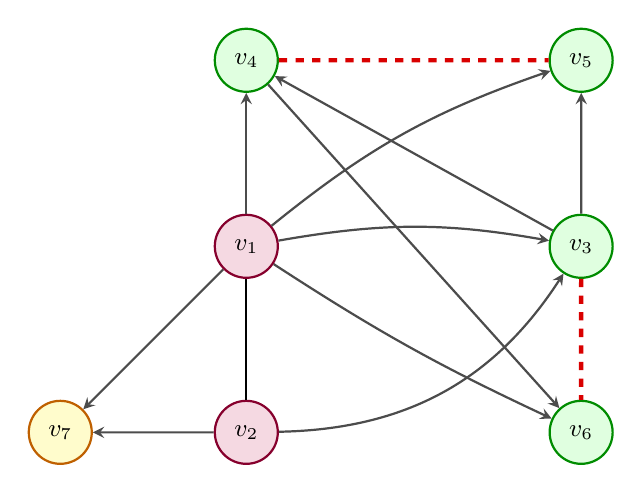
\begin{tikzpicture}[
    scale=1.05,
    >=stealth,
    every node/.style={circle, draw, minimum size=8mm, inner sep=0pt, font=\small},
    seed/.style={fill=purple!15, draw=purple!70!black, line width=0.8pt},
    constrained/.style={fill=green!12, draw=green!55!black, line width=0.8pt},
    free/.style={fill=yellow!20, draw=orange!75!black, line width=0.8pt},
    dep/.style={->, thick, black!70},
    prune/.style={dashed, ultra thick, red!85!black}
]
    % Nodes
    \node[seed] (v1) at (0,0) {$v_1$};
    \node[seed] (v2) at (0,-2.25) {$v_2$};
    \node[constrained] (v3) at (4.05,0) {$v_3$};
    \node[constrained] (v4) at (0,2.25) {$v_4$};
    \node[constrained] (v5) at (4.05,2.25) {$v_5$};
    \node[constrained] (v6) at (4.05,-2.25) {$v_6$};
    \node[free] (v7) at (-2.25,-2.25) {$v_7$};
    
    % Initial clique edge
    \draw[thick] (v1) -- (v2);
    
    % Predecessor arcs (directed)
    \draw[dep] (v1) to[bend left=10] (v3);
    \draw[dep] (v2) to[bend right=28] (v3);

    \draw[dep] (v1) to (v4);
    \draw[dep] (v3) to (v4);
    
    \draw[dep] (v1) to[bend left=10] (v5);
    \draw[dep] (v3) to (v5);
    
    \draw[dep] (v1) to[bend right=4] (v6);
    \draw[dep] (v4) to (v6);

    \draw[dep] (v1) to (v7);
    \draw[dep] (v2) to (v7);
    
    % Pruning edges (dashed red)
    \draw[prune] (v4) to (v5);
    \draw[prune] (v3) to (v6);
\end{tikzpicture}
\caption{Combinatorial predecessor dependency graph and pruning edges for the 7-vertex worked example; node positions are schematic. Directed arcs represent predecessor discretization constraints ($E_D$), dashed red lines represent $E_P = \{\{v_3, v_6\}, \{v_4, v_5\}\}$, purple nodes form $V_0$, green nodes are branch-decision vertices in $B_{\mathrm{c}}$, and the yellow node is the free branch vertex $v_7\in B_{\mathrm{f}}$.}
\label{fig:worked-example}
\end{figure}

The generator supports and associated mirror cliques are listed in Table~\ref{tab:generators}. The constrained rows are ordered as $(v_3,v_4,v_5,v_6)$, and the columns are ordered as $(g_3,g_4,g_5,g_6,g_{C_0},g_{C_1},g_{C_2})$. The free branch bit $v_7$ is intentionally omitted from these constrained masks.

\begin{table}[htbp]
\centering
\caption{Generator supports and mirror cliques for the worked example. Each support mask $S_g$ is a subset of $B_{\mathrm{c}} = \{v_3, v_4, v_5, v_6\}$; the rows define the columns $(g_3,g_4,g_5,g_6,g_{C_0},g_{C_1},g_{C_2})$ of the mask matrix $M$.}
\label{tab:generators}
\begin{tabular}{lcc}
\toprule
Generator & Support Mask ($S_g$) & Mirror Clique ($C_g$) \\
\midrule
$g_3$ & $\{v_3, v_4, v_5, v_6\}$ & $C_0 = \{v_1, v_2\}$ \\
$g_4$ & $\{v_4, v_6\}$ & $C_1 = \{v_1, v_3\}$ \\
$g_5$ & $\{v_5\}$ & $C_1 = \{v_1, v_3\}$ \\
$g_6$ & $\{v_6\}$ & $C_2 = \{v_1, v_4\}$ \\
$g_{C_0}$ & $\{v_3, v_4, v_5, v_6\}$ & $C_0 = \{v_1, v_2\}$ \\
$g_{C_1}$ & $\{v_4, v_5, v_6\}$ & $C_1 = \{v_1, v_3\}$ \\
$g_{C_2}$ & $\{v_6\}$ & $C_2 = \{v_1, v_4\}$ \\
\bottomrule
\end{tabular}
\end{table}

The generator mask matrix is
\[
M=
\begin{bmatrix}
1&0&0&0&1&0&0\\
1&1&0&0&1&1&0\\
1&0&1&0&1&1&0\\
1&1&0&1&1&1&1
\end{bmatrix}.
\]

The active edge set for the constrained subproblem is $F = E_D[L] \cup E_P$. Besides the fixed seed clique edge $\{v_1,v_2\}$, the discretization edges induced on $L$ are
\[
\{v_1, v_3\},\{v_2, v_3\},
\{v_1, v_4\},\{v_3, v_4\},
\{v_1, v_5\},\{v_3, v_5\},
\{v_1, v_6\},\{v_4, v_6\}.
\]
The nonzero labeled active-edge violations are summarized in Table~\ref{tab:violations}.

\begin{table}[htbp]
\centering
\caption{Labeled active-edge violations for each generator. The entry \textnormal{none} means that the generator contributes no row to the labeled violation matrix $V$; the nonzero rows are indexed by $(\{v_4,v_5\},C_1)$ and $(\{v_3,v_6\},C_2)$.}
\label{tab:violations}
\begin{tabular}{lcc}
\toprule
Generator & Violated Active Edge ($e$) & Mirror Label ($C_g$) \\
\midrule
$g_3$ & \text{none} & \text{none} \\
$g_4$ & $\{v_4, v_5\}$ & $C_1$ \\
$g_5$ & $\{v_4, v_5\}$ & $C_1$ \\
$g_6$ & $\{v_3, v_6\}$ & $C_2$ \\
$g_{C_0}$ & \text{none} & \text{none} \\
$g_{C_1}$ & \text{none} & \text{none} \\
$g_{C_2}$ & $\{v_3, v_6\}$ & $C_2$ \\
\bottomrule
\end{tabular}
\end{table}

Thus, with rows ordered as the two active-edge labels $(\{v_4, v_5\},C_1)$ and $(\{v_3, v_6\},C_2)$, the labeled violation matrix is
\[
V=
\begin{bmatrix}
0&1&1&0&0&0&0\\
0&0&0&1&0&0&1
\end{bmatrix}.
\]
Write a generator coefficient vector as $\alpha = (a_3,a_4,a_5,a_6,a_{C_0},a_{C_1},a_{C_2}) \in \mathbb{F}_2^7$. Then the zero-violation condition $V\alpha = 0$, with arithmetic over $\mathbb{F}_2$, is equivalent to
\[
a_4+a_5=0,
\qquad
a_6+a_{C_2}=0.
\]
Hence, $a_4=a_5=t$, $a_6=a_{C_2}=u$, and $a_3,a_{C_0},a_{C_1}$ are free. Applying the mask matrix gives
\[
M\alpha
=
t(m_4+m_5)+u(m_6+m_{C_2})+a_3m_3+a_{C_0}m_{C_0}+a_{C_1}m_{C_1}.
\]
The parameter $u$ changes the generator presentation but not the branch mask, because $m_6=m_{C_2}$. Also $m_3=m_{C_0}$ and $m_4+m_5=m_{C_1}$. Therefore,
\[
\mathcal{K}_F
=
M(\ker V)
=
\left\{
\begin{bmatrix}0\\0\\0\\0\end{bmatrix},
\begin{bmatrix}1\\1\\1\\1\end{bmatrix},
\begin{bmatrix}0\\1\\1\\1\end{bmatrix},
\begin{bmatrix}1\\0\\0\\0\end{bmatrix}
\right\}.
\]
The ranks are
\[
\operatorname{rank}_{\mathbb{F}_2}\begin{bmatrix} M \\ V \end{bmatrix}=4,
\qquad
\operatorname{rank}_{\mathbb{F}_2}(V)=2.
\]
Since $f=1$, the solution count is
\[
\lvert \Xi \rvert = 2^{1+4-2} = 8.
\]
The two independent feasible constrained branch shifts are the mask $\{v_3,v_4,v_5,v_6\}$, obtained from $g_3$ or $g_{C_0}$, and the mask $\{v_4, v_5, v_6\}$, obtained from $g_4\oplus g_5$, or equivalently from the base generator $g_{C_1}$. These generate four feasible constrained codes from a reference solution. The independent free bit at $v_7$ doubles this count, giving eight full feasible branch codes.

\subsection{Concrete Geometric Realization}
\label{sec:example-geometry}

To ground this algebraic structure, we provide a concrete geometric realization in $\mathbb{R}^2$ with exact coordinates. This numerical setup illustrates how the combinatorial conditions established by our theory manifest physically as distance-preserving operations.

\paragraph{Reference Coordinate Embedding.}
We place the initial clique $V_0 = \{v_1, v_2\}$ and the branch decision vertex $v_3$ at
\[
v_1 = (0,0), \quad v_2 = (-2,0), \quad v_3 = (0,2).
\]
The remaining vertices are placed at their reference coordinates:
\[
v_4 = (1, 1), \quad v_5 = (2, 2), \quad v_6 = (2, 0), \quad v_7 = (-1,1).
\]
These coordinates determine the physical edge weights. All discretization distances are positive and can be verified directly: $d_{13} = 2$, $d_{23} = 2\sqrt{2}$, $d_{14} = d_{34} = d_{17} = d_{27} = \sqrt{2}$, $d_{15} = 2\sqrt{2}$, $d_{35} = 2$, $d_{16} = 2$, and $d_{46} = \sqrt{2}$. The two active pruning distances to be tested by our constraint matrices are
\[
d_{36} = \|v_3 - v_6\|_2 = 2\sqrt{2},
\qquad
d_{45} = \|v_4 - v_5\|_2 = \sqrt{2}.
\]
The free vertex $v_7$ contributes only its discretization distances $d_{17}$ and $d_{27}$, which do not appear in the active pruning set $F$ since $v_7 \notin L$.

\paragraph{Physical Reflection and Violation Mechanics.}
We can now trace how individual generator moves deform the embedding and interact with the pruning constraints. First, consider the cone generator $g_3$. The mirror for $v_3$ is the $x$-axis, $\operatorname{aff}(v_1, v_2)$. Activating $g_3$ reflects the downstream cone $\{v_3, v_4, v_5, v_6\}$ across this line. Because all affected vertices are reflected together and the fixed endpoints $v_1,v_2$ lie exactly on the mirror, all discretization and pruning distances are trivially preserved. Similarly, the mirror for $v_7$ is also the $x$-axis. Reflecting $v_7$ to $v_7' = (-1,-1)$ preserves its discretization distances $d_{17}$ and $d_{27}$ and has no contact with the pruning edges. This shows geometrically why the branch decision $v_7$ is completely free, contributing the independent factor $2^f = 2$ to the final solution count.

In contrast, isolated branch shifts that do not belong to the kernel $\ker V$ physically violate the pruning constraints. For instance, the mirror for $v_5$ is the $y$-axis, $\operatorname{aff}(v_1, v_3)$. Mirroring only $v_5$ across the $y$-axis yields $v_5' = (-2, 2)$. While this preserves all discretization distances, it stretches the pruning edge $\{v_4, v_5\}$ to $\|v_4 - v_5'\|_2 = \sqrt{10} \ne \sqrt{2}$, confirming a physical violation. This matches the algebraic violation matrix where $g_5$ has a $1$ in row $(\{v_4,v_5\}, C_1)$. Similarly, the cone generator $g_4$ reflects $v_4$ and its descendant $v_6$ across the $y$-axis, yielding $v_4' = (-1,1)$ and $v_6' = (-2,0)$. This preserves the discretization distance $\{v_4, v_6\}$ and the pruning distance $\{v_3, v_6\}$ (since $v_3$ lies on the $y$-axis mirror), but violates the active edge $\{v_4, v_5\}$ to length $\sqrt{10}$. Lastly, the mirror for $v_6$ is the line $y=x$, $\operatorname{aff}(v_1, v_4)$. Reflecting only $v_6$ gives $v_6' = (0,2)$, which collapses the pruning distance to $v_3$ from $2\sqrt{2}$ to $0$, mapping to the algebraic violation of $g_6$ against $\{v_3,v_6\}$.

\paragraph{Kernel-Induced Cancellation and Dynamic Mirrors.}
The core power of our framework is demonstrated when we apply the nontrivial feasible branch shift $h = \{v_4, v_5, v_6\} \in \mathcal{K}_F$, represented algebraically by the generator combination $g_4 \oplus g_5$ (or equivalently by $g_{C_1}$), where adding the redundant generator pair $g_{C_2} \oplus g_6$ yields the same branch mask. Geometrically, this shift instructs us to reflect $v_4, v_5$, and $v_6$ simultaneously across the $y$-axis ($x=0$), yielding:
\[
v_4' = (-1, 1), \quad v_5' = (-2, 2), \quad v_6' = (-2, 0).
\]
Because all three vertices are reflected by the same isometric reflection $R_{C_1}$ across the $y$-axis, the internal active distance $\|v_4' - v_5'\|_2 = \sqrt{2} = d_{45}$ is preserved. 

The interaction with the dynamic mirror of $v_6'$ reveals the beauty of this cancellation. In the original embedding, $v_6$ is placed using the mirror $\operatorname{aff}(v_1, v_4)$. Under the branch shift, $v_4$ moves to $v_4'$, so the dynamic mirror for the subsequent step rotates to $\operatorname{aff}(v_1, v_4')$, which is the line $y = -x$. The coordinates $v_6' = (-2,0)$ are the exact reflection of the reference $v_6 = (2,0)$ across the $y$-axis. Because $v_6'$ is placed symmetrically with respect to the rotated mirror $y = -x$, the discretization distances are preserved. Crucially, the pruning distance to the fixed vertex $v_3 = (0,2)$ is preserved:
\[
\|v_3 - v_6'\|_2 = \|(0,2) - (-2,0)\|_2 = 2\sqrt{2} = d_{36}.
\]
This coordinate realization illustrates how the algebraic kernel $\ker V$ maps perfectly to viable physical realizations in this system, factoring out the representation redundancies and matching the rank-count prediction.


\section{Scope and Genericity}
\label{sec:scope}

This section records what the theorem does and does not claim.

The 6-vertex example analyzed in Section \ref{sec:example} is a small, reproducible check of the construction: the generator masks, the labeled violation matrix, the ranks, and the final count can all be inspected directly.

The generic mirror separation assumption (Definition \ref{def:mirror-sep}) is essential for the exactness of the rank count. It excludes accidental geometric coincidences. In non-generic configurations, the actual number of solutions can be larger than the generic rank count. This happens when an apparently violating edge is preserved accidentally, for example because a point lies unexpectedly on a reflection mirror. Such cases form a proper algebraic exceptional set of measure zero in the coordinate parameter space. Analogous almost-always qualifications appear in existing DDGP and DMDGP counting results \cite{liberti2014number,abud2024impossible}.

The case $K=1$ requires separate treatment because the algebraic bracket-separation arguments used to establish the generic presentation lemma for $K \ge 2$ degenerate on the line.

\subsection{Unification of the Combinatorial DDGP}
\label{sec:combinatorial-ddgp}

We now check that the rank-count formula agrees with a known positive counting result. 

Abud et al. (2024) introduced the subclass of \emph{Combinatorial DDGP}, defined as those DDGP instances where every predecessor set $U_j$ induces a clique of size $K$ in $G$ \cite{abud2024impossible}. They proved that, for this subclass and in the absence of pruning edges, solution counting is combinatorial and yields exactly $2^{n-K}$ incongruent solutions. This is Corollary 3.6 of Abud et al. and also generalizes the DMDGP no-pruning case.

The rank-count formula includes this result as a direct special case:
\begin{enumerate}
    \item When every predecessor set $U_j$ induces a clique, any active discretization edge $\{a, b\} \in E_D[L_P]$ between predecessors of a vertex has both of its endpoints within the clique.
    \item Consequently, if a generator support crosses the boundary, the fixed endpoint is guaranteed to lie on the mirror clique. Thus, no active edges can be violated under any branch transformations.
    \item The labeled violation matrix $V$ is therefore identically the zero matrix ($V = 0$).
    \item Substituting $V = 0$ into our rank formula:
    \[
    \dim \mathcal{K}_F
    =
    \operatorname{rank}\begin{bmatrix}M\\ 0\end{bmatrix} - \operatorname{rank}(0)
    =
    \operatorname{rank}(M) - 0
    =
    n - K,
    \]
    where $M$ has full rank $n-K$ because the cone generators form a triangular system of masks.
\end{enumerate}
This yields exactly $|\Xi_F| = 2^{n-K}$, recovering the positive result of Abud et al. (2024). Thus the rank-count formula agrees with clique-based DMDGP and Combinatorial DDGP counts while also applying to local non-clique DDGP subproblems satisfying the theorem's hypotheses.

\section{Conclusion}
\label{sec:conclusion}

By reformulating the combinatorial constraints of the Discretizable Distance Geometry Problem (DDGP) in the language of linear algebra over $\mathbb{F}_2$, this work establishes a bridge between local geometric reflections and global counting complexity. The core insight is that the complexity of solution counting under pruning is fundamentally governed by the algebraic interaction of labeled violations. When physical violations are systematically indexed by their corresponding mirror cliques, the space of feasible branch shifts emerges naturally as the projection $\mathcal{K}_F = M(\ker V)$. Whenever a viable reference solution exists and mirror-separation holds, this linear structure determines the total solution count by assigning an independent factor of two to each branch decision that escapes the algebraic reach of the pruning constraints.

This perspective provides a unified explanation for the tractability of classical DMDGP and unpruned DDGP instances, where graph-induced symmetries naturally guarantee full branch viability. In the presence of arbitrary pruning edges, the labeled violation matrix $V$ acts as a precise algebraic filter, identifying exactly which combinations of reflections preserve distance constraints. Crucially, our resulting rank formula cleanly decouples the purely combinatorial structure of the discretization graph from the measure-zero geometric coincidences that characterize degenerate physical embeddings.

Our algebraic framework opens a promising avenue for the design of highly efficient distance geometry algorithms. By shifting the focus from combinatorial search over exponential branch trees to linear operations over $\mathbb{F}_2$, this formulation provides the mathematical foundation for solver paradigms that may reduce branch enumeration. In particular, the algebraic filters developed here can be directly integrated into solvers to detect infeasible branches at early stages, bypassing expensive coordinate computations.

Specifically, future work will focus on exploiting the structured sparsity of the mask matrix $M$ and the labeled violation matrix $V$ to construct and solve the associated $\mathbb{F}_2$ systems efficiently for large-scale discretization networks. Such advancements hold the potential to significantly accelerate distance geometry solvers, demonstrating the power of finite-field linear algebra to drastically reduce the computational complexity of spatial reconstruction problems.

\bibliographystyle{plain}
\bibliography{references}

\end{document}
